\documentclass{beamer}
\usepackage{graphicx}
\usepackage{amsmath}
\usepackage{listings}

\lstdefinestyle{mystyle}{   
	commentstyle=\color{codegreen},
	keywordstyle=\color{magenta},
	numberstyle=\tiny\color{codegray},
	stringstyle=\color{codepurple},
	basicstyle=\small,                    
	keepspaces=true,                                  
	showspaces=false,                
	showstringspaces=false,
	showtabs=false,                  
	tabsize=2
}

\lstset{style=mystyle}

\lstset{language=html}
\usepackage{array}
\usepackage{biblatex}
\usepackage{tikz}
\usepackage{smartdiagram}
\addbibresource{rapport.bib}
\usepackage{hyperref}
\graphicspath{{~/templates/}, {../images/}}
\usetheme{Hannover}

\addtobeamertemplate{navigation symbols}{}{%
	\usebeamerfont{footline}%
	\usebeamercolor[fg]{footline}%
	\hspace{1em}%
	\insertframenumber/\inserttotalframenumber
}


\begin{document}
	
	\begin{frame}
		
		\centering
		\vspace{4em}
		\textbf{Mémoire de Stage de 4e année}\\
		\vspace{2em}
		\textbf{\LARGE FL-Minifer}\\
		\textbf{\large A Tool To Minify and Unify AdBlocker’s Filter Lists}\\
		\vspace{3em}
		
		\begin{tabular}{ c c }
			
\includegraphics[width=0.4\textwidth]{logoInria.jpg} & 
\includegraphics[width=0.5\textwidth]{logospirals.png}\\
		\end{tabular}
	
		\vspace{4em}
		\begin{tabular}{m{0.45\textwidth} p{0.45\textwidth}}
			NEUS Maxence & \hspace{\fill}2022
		\end{tabular}
		
	\end{frame}

	\section{Contexte du stage}
	\subsection{Inria}
	
	\begin{frame}
		\frametitle{L'Inria}
		\centering
		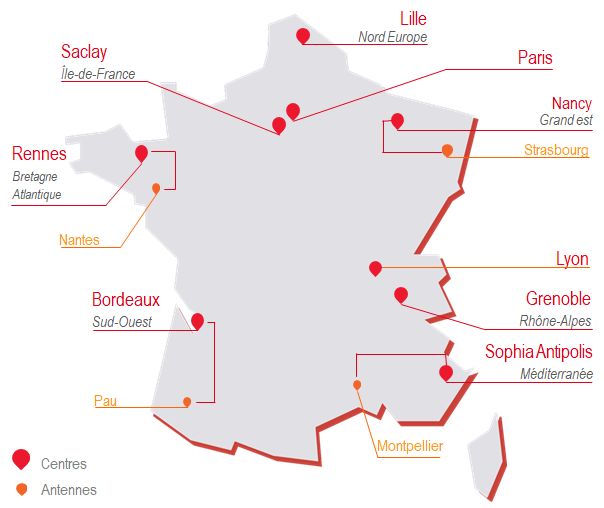
\includegraphics[width=0.4\textwidth]{cartecentres.png}
		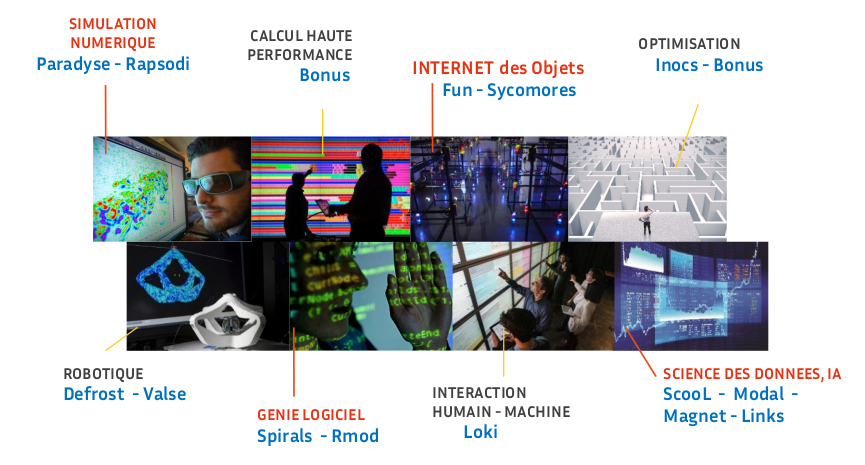
\includegraphics[width=0.8\textwidth]{equipesCentre.png}
	\end{frame}

	\subsection{Le projet AmIUnique}
	\begin{frame}
		\frametitle{Browser Fingerprinting}
		\begin{tabular}{m{0.5\textwidth} m{0.1\textwidth} m{0.3\textwidth}}
			\begin{itemize}
				\item Configuration navigateur
					\begin{itemize}
						\item Version
						\item Polices par défaut
						\item ... 
					\end{itemize}
				\item Hardware
					\begin{itemize}
						\item Résolution écran
						\item RAM
						\item ... 
					\end{itemize}
			\end{itemize} & \huge \textrightarrow & Identificateur unique
		\end{tabular}
	\end{frame}

	\begin{frame}{AmIUnique}
		\begin{itemize}
			\item Pour l'utilisateur
			\begin{itemize}
				\item Montre les composantes de la fingerprint et propose des explications sur le démarche
				\color{lightgray}
				\item Incorpore un algorithme en cours de développement permettant de déterminer  les listes de filtres d'adBlockers installées
			\end{itemize}
			\color{lightgray}
			\item Pour la recherche
			\begin{itemize}
				\color{lightgray}
				\item Créer un dataset de fingerprints pour évaluer les éléments les plus identifiables et mesurer l'impacte de contremesures
				\item Traquer les changements dans la fingerprint au cours du temps
			\end{itemize}
		\end{itemize}
	\end{frame}

	\begin{frame}{AmIUnique}
		\begin{itemize}
			\item Pour l'utilisateur
			\begin{itemize}
				\color{gray}
				\item Montre les composantes de la fingerprint et propose des explications sur le démarche
				\color{black}
				\item Incorpore un algorithme en cours de développement permettant de déterminer  les listes de filtres d'adBlockers installées
			\end{itemize}
			\color{lightgray}
			\item Pour la recherche
			\begin{itemize}
				\color{lightgray}
				\item Créer un dataset de fingerprints pour évaluer les éléments les plus identifiables et mesurer l'impacte de contremesures
				\item Traquer les changements dans la fingerprint au cours du temps
			\end{itemize}
		\end{itemize}
	\end{frame}

	\begin{frame}{AmIUnique}
		\begin{itemize}
			\color{gray}
			\item Pour l'utilisateur
			\begin{itemize}
				\color{gray}
				\item Montre les composantes de la fingerprint et propose des explications sur le démarche
				\item Incorpore un algorithme en cours de développement permettant de déterminer  les listes de filtres d'adBlockers installées
			\end{itemize}
			\color{black}\item Pour la recherche
			\begin{itemize}
				\item Créer un dataset de fingerprints pour évaluer les éléments les plus identifiables et mesurer l'impacte de contremesures
				\item \color{lightgray} Traquer les changements dans la fingerprint au cours du temps
			\end{itemize}
		\end{itemize}
	\end{frame}

	\begin{frame}{AmIUnique}
		\begin{itemize}
			\color{gray}
			\item Pour l'utilisateur
			\begin{itemize}
				\color{gray}
				\item Montre les composantes de la fingerprint et propose des explications sur le démarche
				\item Incorpore un algorithme en cours de développement permettant de déterminer  les listes de filtres d'adBlockers installées
			\end{itemize}
			\color{black} \item Pour la recherche
			\begin{itemize}
				\color{gray}
				\item Créer un dataset de fingerprints pour évaluer les éléments les plus identifiables et mesurer l'impacte de contremesures
				\item \color{black} Traquer les changements dans la fingerprint au cours du temps
			\end{itemize}
		\end{itemize}
	\end{frame}

	\begin{frame}{Filter lists}
		\framesubtitle{Création des tests}
		\begin{center}
			\smartdiagramset{back arrow disabled=true,text width=2cm, font=\fontsize{6pt}{12pt}\selectfont}
			\smartdiagram[flow diagram:horizontal]{Récupération des listes, Génération HTML, Filtre les superpositions, Mise à jour base de tests}
		\end{center}
	\end{frame}

	\begin{frame}[fragile]{Filter Lists}
		\framesubtitle{Page de test}
		\begin{lstlisting}
<img src='source' style='visibility: hidden' />
		\end{lstlisting}
	
		\begin{center}
			\huge \textdownarrow \\
			\vspace{1em}
			\normalsize Test la visibilité de l'élément sur la page
		\end{center}
	\end{frame}

	\section{Travaux effectués}
	\subsection{Extension}
	
	\begin{frame}[fragile]{Extension Chrome}
		\framesubtitle{Expérimentations}
		\centering
		La règle \verb|###ad-boxes| est inclue dans \textbf{EasyList}\\
		\vspace{1em}
		
		\verb|##| \textrightarrow Bloquer les éléments avec le CSS \verb*|#ad-boxes|
		
		C'est à dire avec un id de \verb*|ad-boxes|
		
	\end{frame}
	
	\begin{frame}[fragile]{Extension Chrome}
		\framesubtitle{Expérimentations}
				
		\begin{lstlisting}
<img id='ad-boxes'/>
		\end{lstlisting}
	\end{frame}

	\begin{frame}[fragile]{Extension Chrome}
		\framesubtitle{Expérimentations}
		\includegraphics[width=\textwidth]{chrome.png}
	\end{frame}

	\begin{frame}[fragile]{Extension Chrome}
		\framesubtitle{Expérimentations}
		\centering
		
		\texttt{@@||www.google.*/search?\$generichide}\\
		\vspace{1em} \color{lightgray}
		\texttt{@@} \textrightarrow règle d'exception\\
		\vspace{1em}
		\texttt{||} spécifie le domaine\\
		\vspace{1em}
		\texttt{\$generichide} ici empêche tout blocage venant du domaine 
	\end{frame}
	
	\begin{frame}[fragile]{Extension Chrome}
		\framesubtitle{Expérimentations}
		\centering
		
		\texttt{@@||www.google.*/search?\$generichide}\\
		\vspace{1em}
		\texttt{@@} \textrightarrow règle d'exception\\
		\vspace{1em}\color{lightgray}
		\texttt{||} spécifie le domaine\\
		\vspace{1em}
		\texttt{\$generichide} ici empêche tout blocage venant du domaine 
	\end{frame}

	\begin{frame}[fragile]{Extension Chrome}
		\framesubtitle{Expérimentations}
		\centering
		
		\texttt{@@||www.google.*/search?\$generichide}\\
		\vspace{1em}\color{gray}
		\texttt{@@} \textrightarrow règle d'exception\\
		\vspace{1em}\color{black}
		\texttt{||} spécifie le domaine\\
		\vspace{1em}\color{lightgray}
		\texttt{\$generichide} ici empêche tout blocage venant du domaine 
	\end{frame}
	
	\begin{frame}[fragile]{Extension Chrome}
		\framesubtitle{Expérimentations}
		\centering
		
		\texttt{@@||www.google.*/search?\$generichide}\\
		\vspace{1em}\color{gray}
		\texttt{@@} \textrightarrow règle d'exception\\
		\vspace{1em}
		\texttt{||} spécifie le domaine\\
		\vspace{1em}\color{black}
		\texttt{\$generichide} ici empêche tout blocage venant du domaine 
	\end{frame}

	\begin{frame}[fragile]{Extension Chrome}
		\framesubtitle{Expérimentations}
		\centering
		
		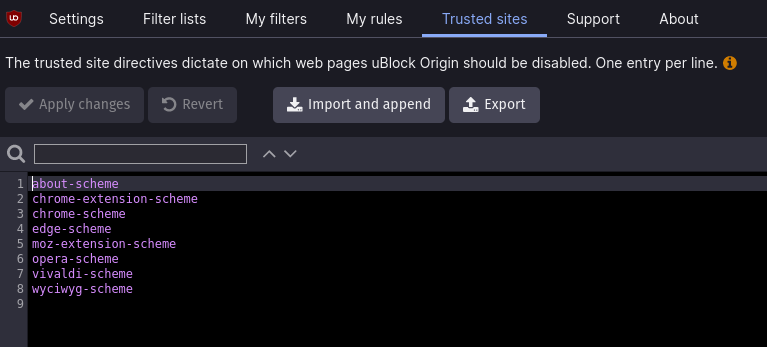
\includegraphics[width=\textwidth]{trustedsites.png}
	\end{frame}

	\begin{frame}[fragile]{Extension Chrome}
		\framesubtitle{Plan pour le suite}
		\centering
		\begin{tabular}{m{0.45\textwidth} m{0.45\textwidth}}
			Network Rules & Cosmetic Rules \\
			\hline
			\begin{itemize}
				\item Récupérer le code \textit{AmIUnique}
				\item Transforme l'interface express avec des messages Chrome
				\item Gérer la base de donnée depuis Chrome
			\end{itemize} & 
			\begin{itemize}
				\item Prendre en compte les Trusted sites et règles d'exception
				\item Si rien n'est bloqué, alors le test est ignoré
			\end{itemize}
		\end{tabular}
		\vspace{2em}
		Package le code dans un plugin
		
	\end{frame}

	\begin{frame}{References}
		\nocite{*}
		\printbibliography
	\end{frame}

\end{document}